% !TeX root = ../main.tex
% Add the above to each chapter to make compiling the PDF easier in some editors.

\chapter{Gen6D: Formal Description}\label{chapter:gen6d_formal_description}

\section{Overview of the Network}
After conducting a scientific literature search, we decided on an interesting model known as Gen6D: Generalizable Model-Free 6-\ac{DoF} Object Pose Estimation from RGB Images \cite{liu2023gen6d}. This architecture is fed with reference and query images, and operates in a relatively straightforward manner, comprising three stages shown in Figure~\ref{fig:fig0}. Initially, there's the detector, which, as its name suggests, detects the object in the query image. Next is the viewpoint selection, which selects reference images that have the closest viewing angle to the detected object in the query image by using a similarity score. Finally, there's the pose refiner, which enhances the accuracy of the estimated pose through a 3D volume-based process. We have compiled a table summarizing the advantages and disadvantages for a clearer understanding:

\begin{table}[htpb]
  \caption[Example table]{Summary of Gen6D}\label{tab:sample}
  \centering
  \small
  \begin{tabular}{l | l}
    \toprule
      Pros & Cons \\
    \midrule
      Generalizability & Limited by Reference Image Quality \\
      Model-Free & Everyday Life Objects Training Data \\
      Simple Input Requirements & Difficulty with Symmetric Objects \\
      Robustness to Background Clutter & Dependence on Initial Detection and Selection \\
      Effective in Diverse Environments & Potential Challenges with Severe Occlusions \\
      Competitive Performance & Computationally Intensive \\
    \bottomrule
  \end{tabular}
  \label{tab:tab}
\end{table}

\begin{figure}[ht]
  \centering
  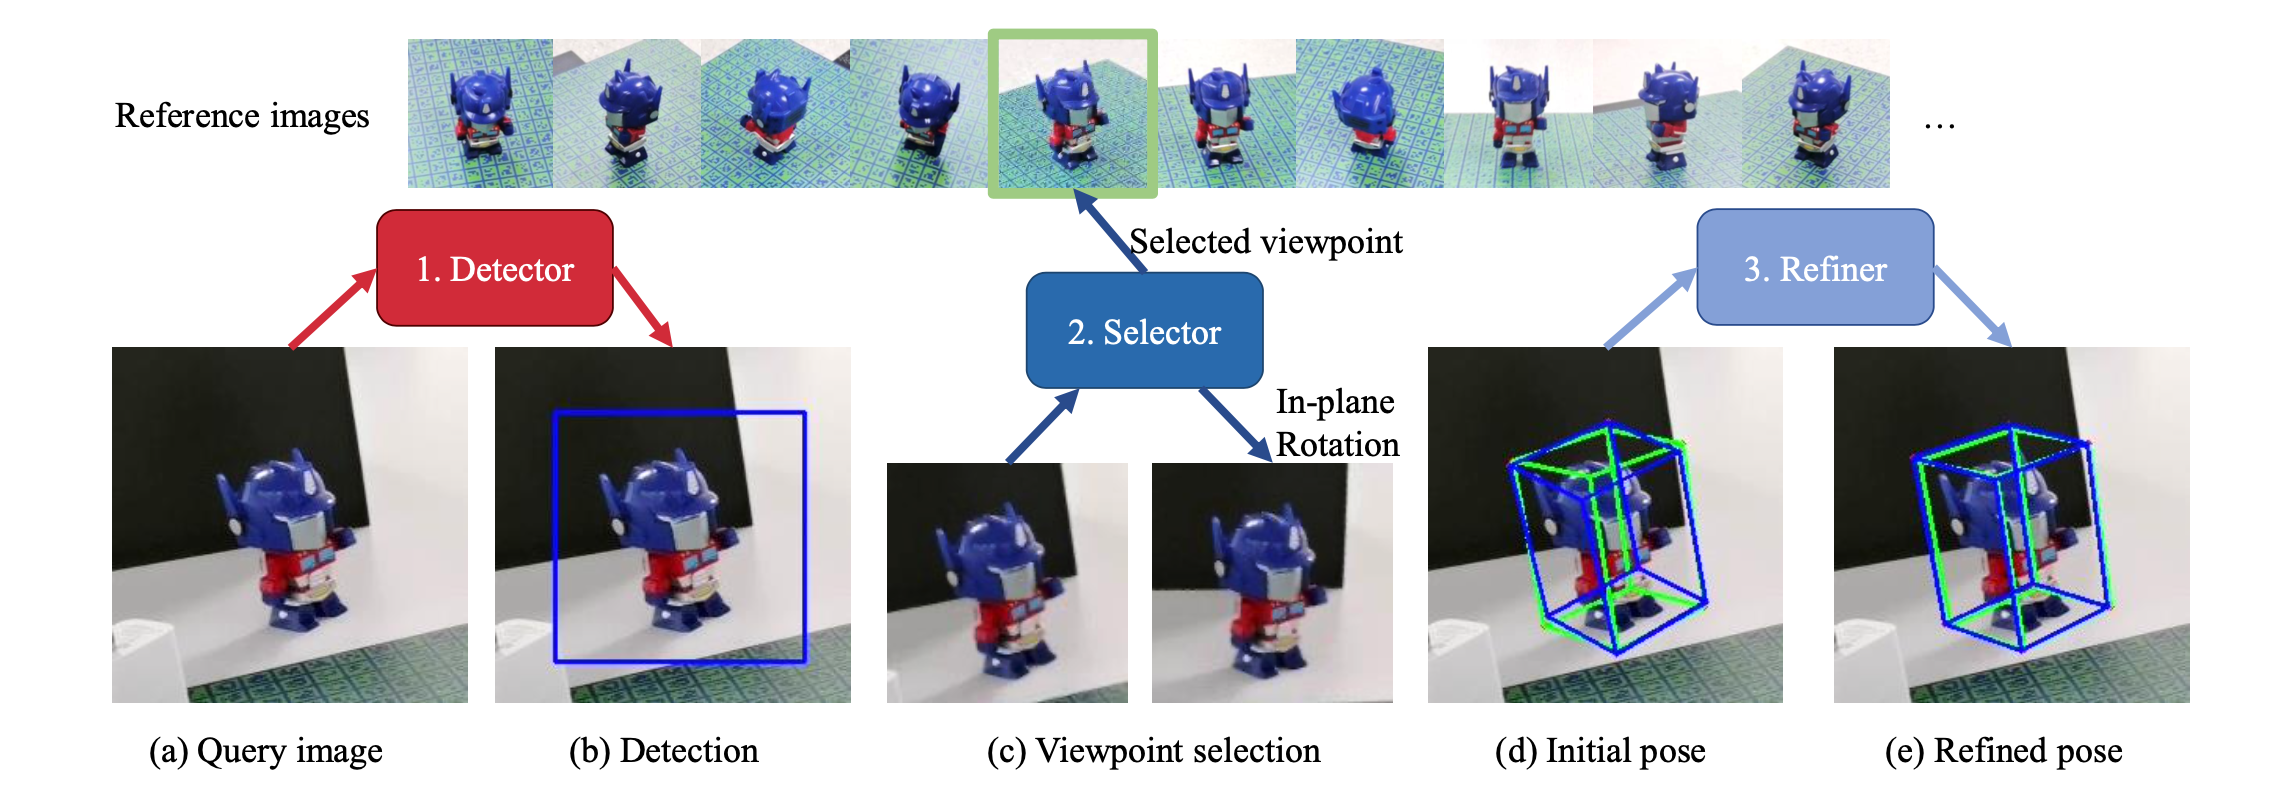
\includegraphics[width=\textwidth]{data/gen6d1.png}
  \caption{Overview of Gen6D, image sourced from Gen6D's research paper.}
  \label{fig:fig0}
\end{figure}

\section{Detection}
\fancyhead[C]{\small\textsc{2.2. Detection}}

In the detection phase, the initial step involves resizing both reference and query images. The reference images are resized to a dimension of ($128 \times 128$), with the object centered. The query images are resized at various predefined scales. Subsequently, all the resized images are processed through a \ac{VGGNet}, which essentially functions as a deep convolutional network for extracting feature maps.

Following this, the feature maps from the reference images are utilized as convolutional kernels to convolve with one of the query images, resulting in the generation of a score map. Leveraging the multi-scale score map, we perform regression to obtain a heat map and a scale map. The final 2D detection is acquired by identifying the maximum value in the heat map, which provides the object's center coordinates, while the scale $s$ is obtained from the same location in the scale map, by this way determining the size of the 2D bounding box.

\begin{figure}[ht]
  \centering
  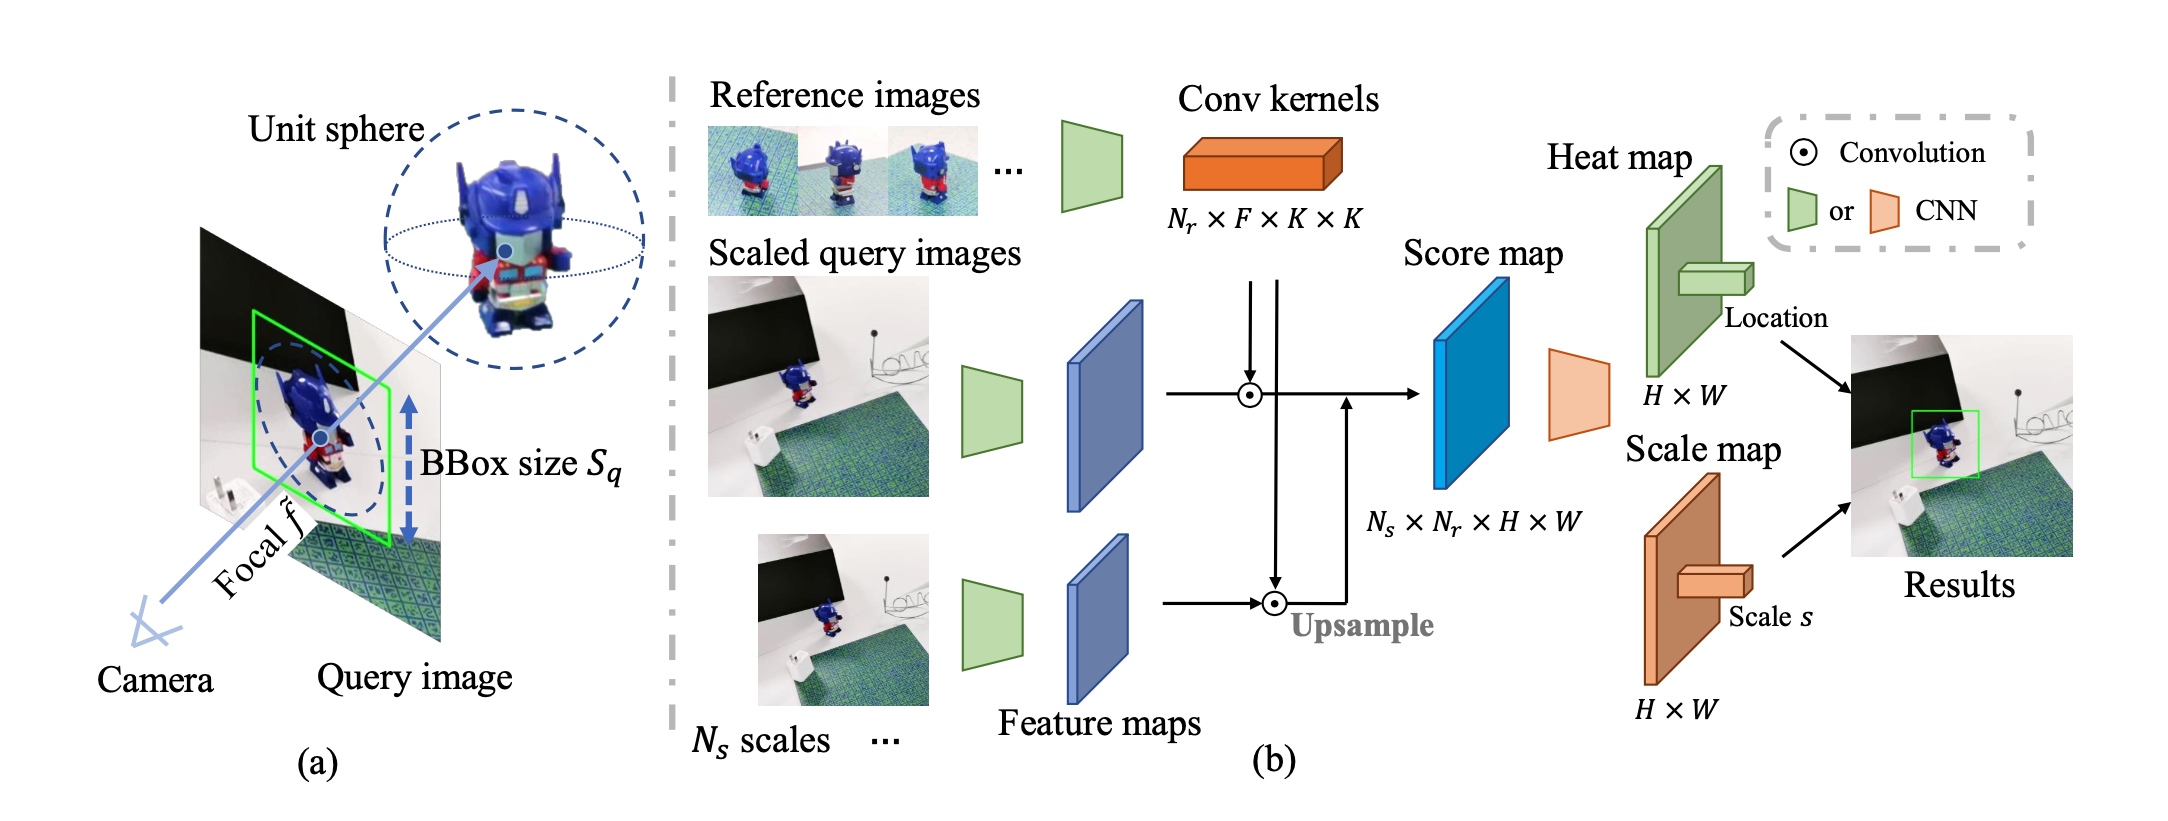
\includegraphics[width=\textwidth]{data/gen6d2.png}
  \caption{Architecture of the detector, image sourced from Gen6D's research paper.}
  \label{fig:fig1}
\end{figure}

\section{Viewpoint Selection}
%\fancyhead[C]{\small\textsc{2.3. Viewpoint Selection}}

During the viewpoint selection phase, we begin by applying predefined rotations to the reference images to accommodate in-plane rotation variations. After that, we once again extract feature maps from both the query image, which has been cropped based on the detection results, and the rotated reference images.

Next we calculate the element-wise product of the query image's features with those of each rotated reference image, yielding a correlation score map. These scores are then inputted into a similarity network, which produces a similarity score and the relative in-plane rotation.

It's worth highlighting that within the similarity network, the authors have implemented global normalization and incorporated a transformer to facilitate information sharing among the reference images.

\begin{figure}[ht]
  \centering
  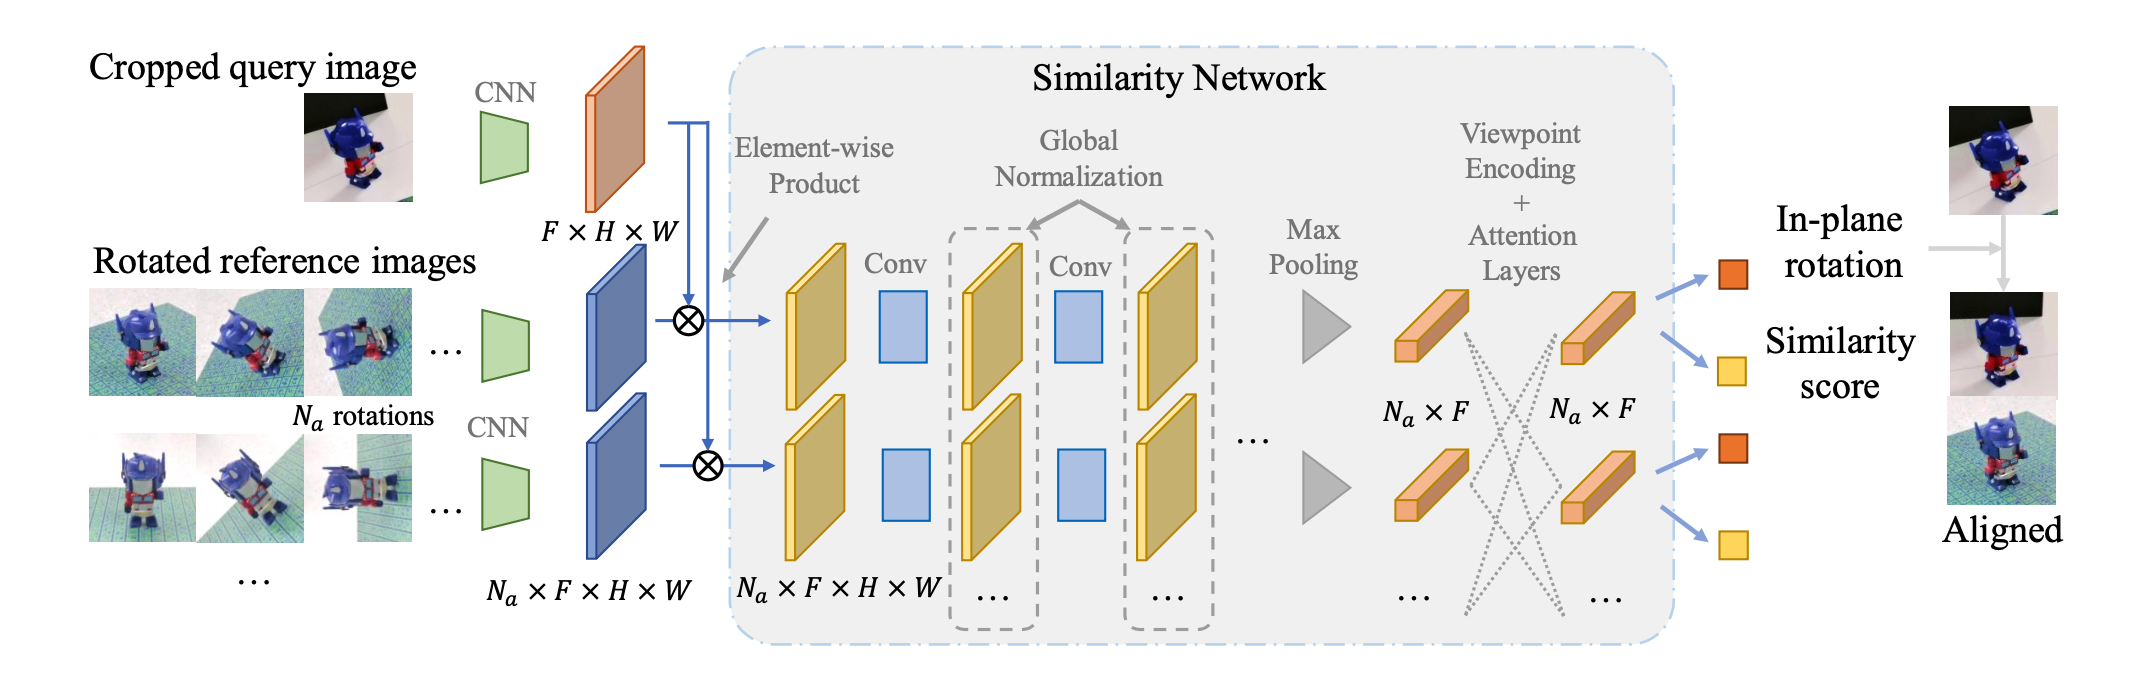
\includegraphics[width=\textwidth]{data/gen6d3.png}
  \caption{Architecture of the viewpoint selector, image sourced from Gen6D's \\ research paper.}
  \label{fig:fig2}
\end{figure}

\section{Pose Refinement}

From the two previous stages, we have an initial coarse object pose. 
In this refinement process, we one last time extract feature maps from the selected reference images using a 2D \ac{CNN}. Afterwards, these feature maps are unprojected into the 3D volume, and we compute their mean and variance, used as features associated with the volume vertices.

Similarly, for the query image, we perform the same process but utilize the input pose. The unprojected query image features are then concatenated with the previously obtained mean and variance features.

At the end, we have a 3D \ac{CNN} that operates on the concatenated feature set of the volume, so as to predict a pose residual that updates the input pose. We iterate through the loop three times, which has been determined empirically as the optimal number of steps, in order to enhance the accuracy of the estimated pose.


\begin{figure}[ht]
  \centering
  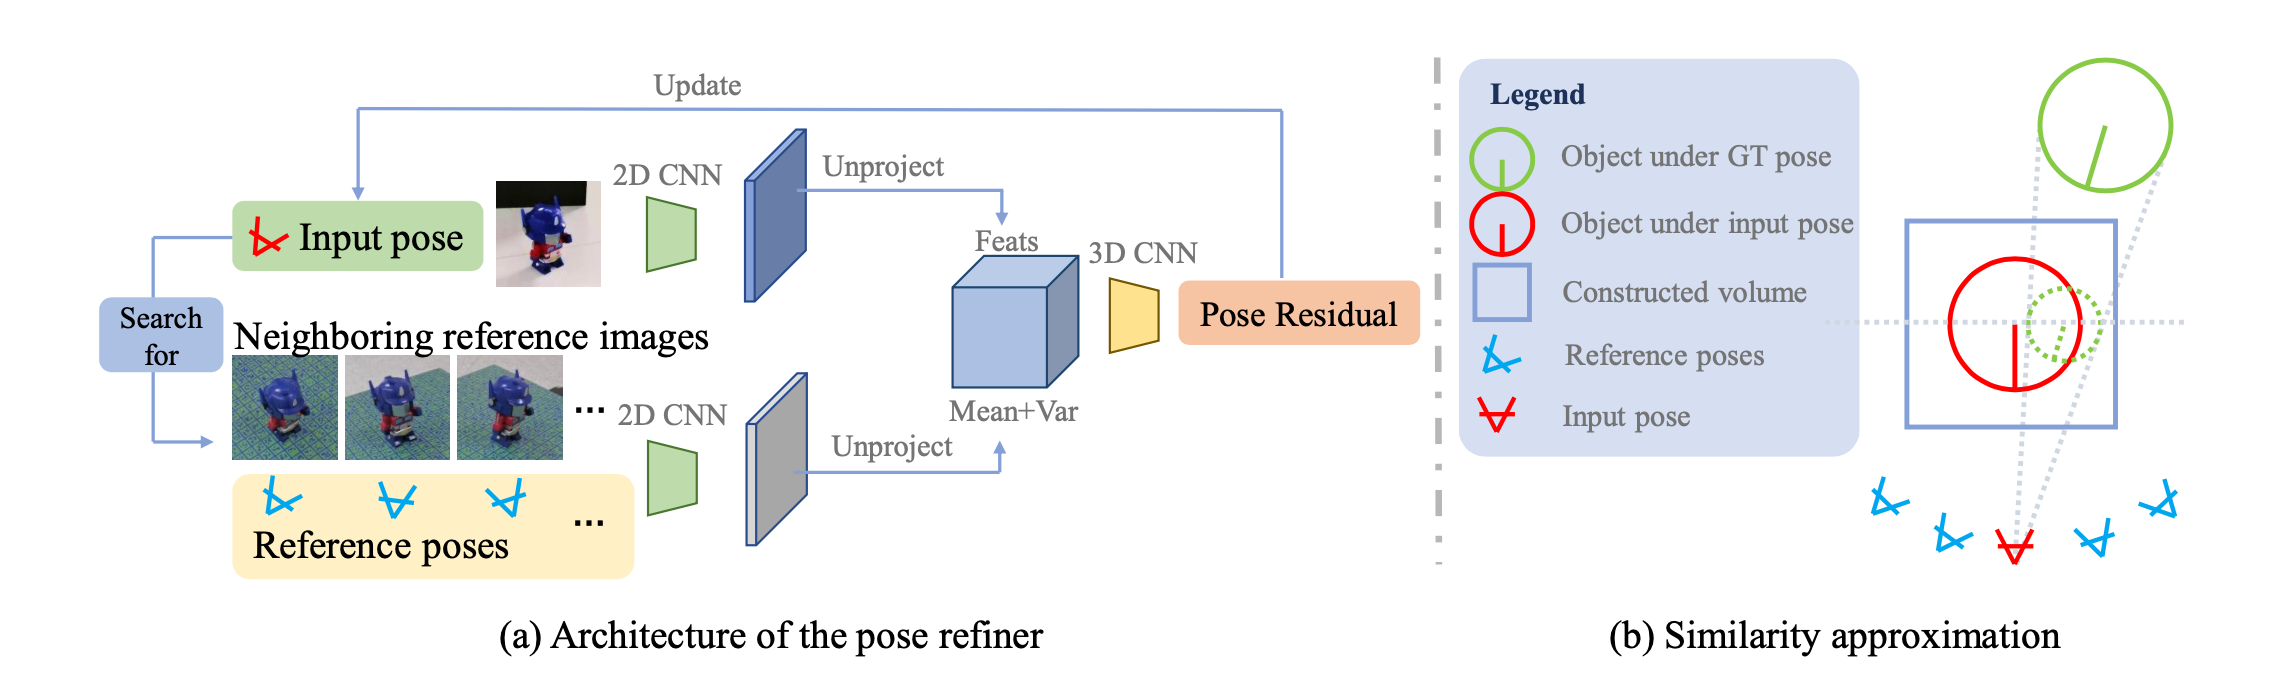
\includegraphics[width=\textwidth]{data/gen6d4.png}
  \caption{Architecture of the pose refiner, image sourced from Gen6D's research paper.}
  \label{fig:fig3}
\end{figure}

\fancyhead[C]{\small\textsc{2.4. Pose Refinement}}